% Name: Matrix multiplication
% Description: A row of A and a column of B highlighted with the entry of the product they make.
% Tags: matrix multiplication, linear algebra, row times column

\usetikzlibrary{matrix, fit, backgrounds, positioning}

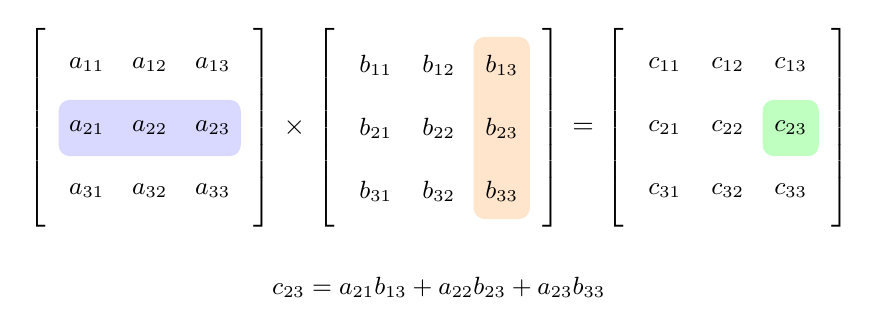
\begin{tikzpicture}[
  mat/.style={
    matrix of math nodes, left delimiter={[}, right delimiter={]},
    nodes={minimum size=7mm, font=\small}, column sep=1mm, row sep=1mm,
  },
]
  \matrix[mat] (A) {
    a_{11} & a_{12} & a_{13} \\ a_{21} & a_{22} & a_{23} \\ a_{31} & a_{32} & a_{33} \\
  };
  \node[right=3mm of A] (times) {$\times$};
  \matrix[mat, right=3mm of times] (B) {
    b_{11} & b_{12} & b_{13} \\ b_{21} & b_{22} & b_{23} \\ b_{31} & b_{32} & b_{33} \\
  };
  \node[right=3mm of B] (eq) {$=$};
  \matrix[mat, right=3mm of eq] (C) {
    c_{11} & c_{12} & c_{13} \\ c_{21} & c_{22} & c_{23} \\ c_{31} & c_{32} & c_{33} \\
  };
  \begin{scope}[on background layer, every node/.style={rounded corners, inner sep=0pt}]
    \node[fill=blue!15, fit=(A-2-1)(A-2-3)] {};
    \node[fill=orange!20, fit=(B-1-3)(B-3-3)] {};
    \node[fill=green!25, fit=(C-2-3)] {};
  \end{scope}
  \node[below=5mm of B, font=\small] {$c_{23} = a_{21} b_{13} + a_{22} b_{23} + a_{23} b_{33}$};
\end{tikzpicture}
